\section{Scenarios}
\label{sec:scenarios}

In this work, we explore the deployment of advanced reactors in the future
energy landscape of the \gls{usa}. As the landscape evolves, compounding
factors will drive the actual deployment of these reactors in ways this work
does not capture. The value of energy system modeling and this type of
transition scenario is to understand the implications of deployment compared
with and measured relative to business-as-usual cases with similar
approximations.

We use this chapter to explore the deployment schemes we have
implemented---outlined in Table \ref{tab:deployment_schemes}---, and the demand
growth scenarios we have considered---outlined in Table
\ref{tab:demand_scenarios}. In Appendix \ref{sec:considered_deployment_schemes}
we will discuss two additional deployment schemes that we implemented, but
not incorporated as they are more useful for problems not considered herein.

\begin{table}[H]
    \centering
    \caption{Deployment Schemes}
    \label{tab:deployment_schemes}
    \begin{tabular}{p{0.15\linewidth} p{0.27\linewidth} p{0.50\linewidth}}
        \hline
        \textbf{Status} & \textbf{Scheme} & \textbf{Description} \\
        \hline
        \multirow{4}{*}{Incorporated} & Greedy Deployment & Deploy the largest
        reactor first at each time step, fill in the remaining capacity with
        the next smallest, and so on. \\
        & Random Deployment & Uses a date and hour as seed to sample the
        reactors list randomly. \\
        & Initially Random, Greedy Deployment & Randomly deploys reactors until
        a reactor bigger than the remaining capacity is proposed for each year,
        then fills the remaining capacity with a greedy algorithm. \\
        Single Reactor & A single reactor model is deployed as the existing fleet is decommissioned.\\
        \hline
        \multirow{2}{*}{Not Incorporated} & Capped Deployment & There is a
        single-number capacity for one or more of the reactor models. \\
        & Pre-Determined Distribution Deployment & One or more reactors have a
        preset distribution, and a smaller capacity model fills in the gaps. \\
        \hline
    \end{tabular}
\end{table}

We apply these deployment schemes to demand growth scenarios based on two
predictions of future energy demand. The \gls{eia} publishes demand expansion
projections for the totality of \gls{usa} \cite{eia_aeo_2023}. As we have
discussed, the administration has refrained from publishing AEO 2024 in light
of recent accelerations in demand growth. Our assumptions for the low-growth
scenarios are that the relative percentage of nuclear power remains constant
and that the relative performance of the various fuel cycle metrics we simulate
will remain constant. The \gls{doe} Liftoff Report
\cite{julie_liftoff_pathways_2024} does not reflect this constant percentage
assumption for nuclear power in their demand scenarios, which are specific to
nuclear deployment increases and the number is agnostic to the total increase.

\begin{table}[H]
    \centering
    \caption{Demand Growth Scenarios}
    \label{tab:demand_scenarios}
    \begin{tabular}{c c c}
        \hline
        \textbf{Demand Growth} & \textbf{Year-to-Year Increase} & \textbf{Source}\\
        \hline
        No growth & 0\% & na\\
        Low growth & 0.17\%, 0.5\%, 1\%, & \cite{eia_aeo_2023}\\
        High growth & 3.5\%, 5.6\% & \cite{julie_liftoff_pathways_2024}\\
        \hline
    \end{tabular}
\end{table}

Each growth scenario is deployed under two regimes: 1) the reactors are never
fueled with \gls{leup}; 2) the \gls{mmr} and \gls{xe} reactors are fueled with
\gls{leup} until 2040, when they move to \gls{haleu}. \glspl{mmr} deployed
before this fuel transition will continue to use \gls{leup} fuel until the end
of their lifetime as they do not refuel; however, the \gls{xe} reactors will
refuel with \gls{leup} until 2040, when they will refuel with \gls{haleu}. The
AP1000 reactors will continue to use \gls{leu} fuel throughout the simulation.

Under each regime, each growth scenario is met by deploying reactors using the
schemes outlined in Table \ref{tab:deployment_schemes}. We will discuss the
results of these deployment schemes in the following sections. We will also
discuss the limitations of this work and propose future work. Regardless of the
regime, each deployment scheme will attempt to deploy reactors to meet the
capacity outlined in Figure \ref{fig:dep_goals}.

\begin{figure}[H]
    \centering
    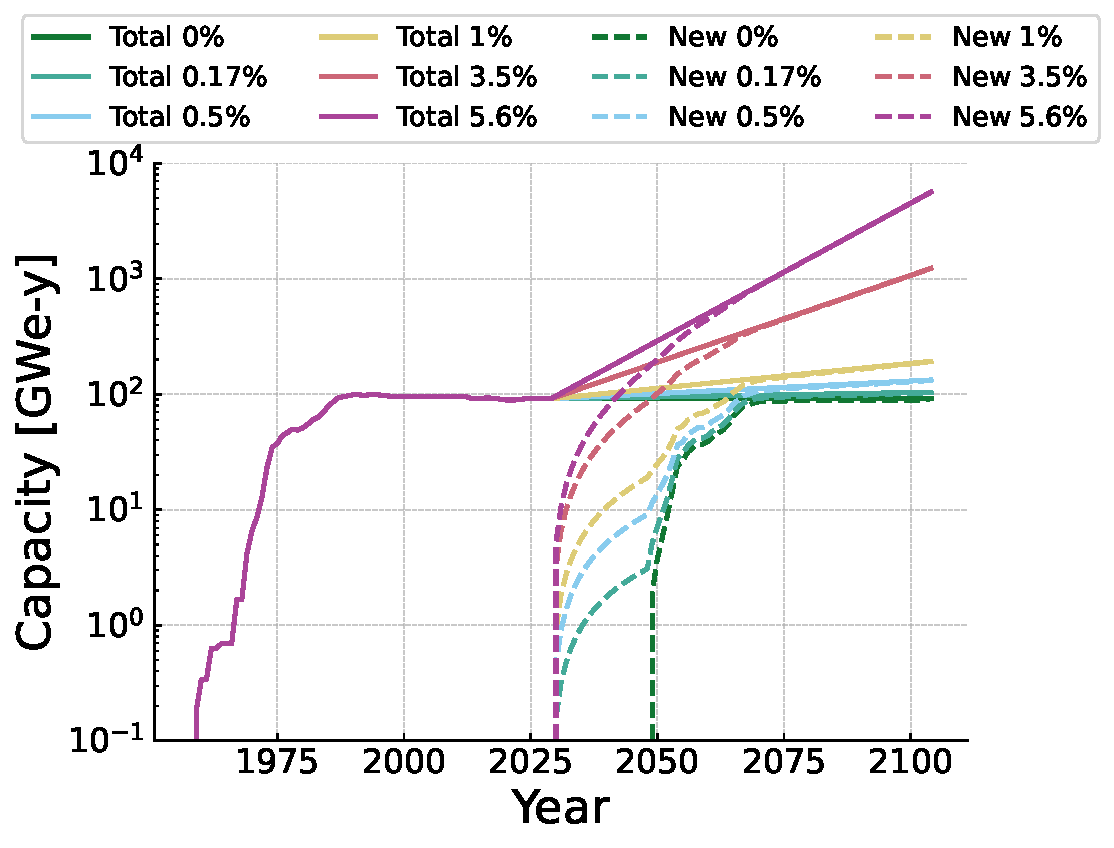
\includegraphics[scale=0.75]{images/results/deployment_calcs/total_new_capacity_scenarios.pdf}
    \caption{Total and new nuclear capacity deployed in each scenario}
    \label{fig:dep_goals}
\end{figure}

As shown, advanced reactors (for the purposes of this work the designs are the:
\gls{mmr}, \gls{xe}, and AP1000) begin deployment in 2030. While this is an
aggressive deployment schedule, \cite{bachmann_thesis_2023} established that
the precise deployment start did not significantly impact the total results for
this type of analysis and could reasonably serve as an upper bound of
deployment. The business-as-usual or, as we will refer to it, no growth
scenario does not require the deployment of a new nuclear reactor until just
before 2050, whereas the other scenarios understandably commence deployment in
2030. As we have presented the capacity on a logarithmic plot, the linear
appearance of the data belies the compounding effect that the year-to-year
percentage growth requires.

We will focus on the results of the no growth and $3.5\%$ scenarios, and the results for the other scenarios are available in Appendix \ref{ch:additional_results}.